
\documentclass[11pt, a4paper]{report}
\usepackage{graphicx}
\usepackage{fullpage}
\usepackage{url}
\usepackage{listings}
\usepackage{hyperref}
\pagestyle{headings}

\headsep = 25pt
\begin{document}

\title{\Huge IndividualTesting Report }
\author{Yufeng Bai\\ \\ID: 1600095}
\date{20 October 2012}
\maketitle
\pagebreak
\oddsidemargin -0.5 cm
\evensidemargin -0.5 cm
\textwidth 15 cm
\topmargin -1.2 cm
\textheight 25 cm
\tableofcontents

\chapter{Introduction of the Test Plan}
In this project, I am be chosen to do the GUI button, speed slider tests and some physical tests. The GUI is used on the host system side, which is used to implement the manual control, map operation and robot status displaying. The scope of my GUI test covers these parts below:
\section{GUI Button test introduction}
My GUI button test is mainly used to test the buttons of the GUI in different situation.
\begin{enumerate}
\item The default button. When the GUI is running, if the user does not do the further operation, some buttons are not allowed to be pressed.
\item The new map initial button. When the map is created, there are some buttons are active, but some others are still inactive. 
\item The bluetooth connection button. When the bluetooth connection is successful, there are some buttons are active, but some others are still inactive. The bluetooth connection button include the mode change button. When the mode change button is active, the current mode button is not allowed to be pressed again.    
\end{enumerate} 
\section{Speed Slider test}
The speed slider test is used to test whether the value of the speed slider matches the value of the current speed. Meanwhile, it is also test whether or not this value is able to demonstrate on the information board. 
\section{Physical test}
The physical test is used to test the accuracy of the robot. In physical test, i mainly test whether the current program parameters are accurate to control the robot. In my physical test case, I mainly include three movement operation of the robot.  
\begin{enumerate}
\item Forward Operation. Using GUI to control the forward movement(it means move to the north of the map) of the robot, mainly check whether or not the robot is able to move one pixel when user presses forward button every one time.
\item TurnLeft Operation. Using GUI to control the turnLeft movement of the robot. When user uses the GUI to let the robot turn left, I need to make sure the robot is able to turn left 90 degrees. 
\end{enumerate}
\chapter{Test Plan and Specific Test Case}
\section{The function or class I need to test in different situation}
\begin{enumerate}
\item Since the GUI is an entirety, it is hard to test one method, I plan to test the all relevant methods for one button.  The test functions include All functions and class about the Jbutton auto, manual, addNew, loadMap, up, down, left, right, turnLeft, turnRight, bluetoothConnection in the FIle LEGOGUI.  
\item Test the functions and class which is relevant to the Slider. Testing the value of the speed slider and the value of the current speed.
\item For the Physical test, I presume i do not know the specific program of the robot, what i need to do is to test the specific location of the robot after operating by GUI. 
\end{enumerate}
\section{Testing Tool and Operating System}
\begin{itemize}
\item Eclipse SDK for java developer with JUnit test
\item Version: 3.7.2
\item Build id: M20120208-0800
\item Operating System: OS X 10.8.2(12C60)
\end{itemize}
\section{Test1: Default Button}
\subsection{Test method}
\subsection{Description:}
When the GUI is running, there are some buttons allowing to press and some buttons not allowing to press. I plan to use Jbutton.isEnabled method to test whether not these buttons are able to work correctly. The button with colour tray is not allowed to be pressed.The initial GUI displays below:
 \begin{center}
 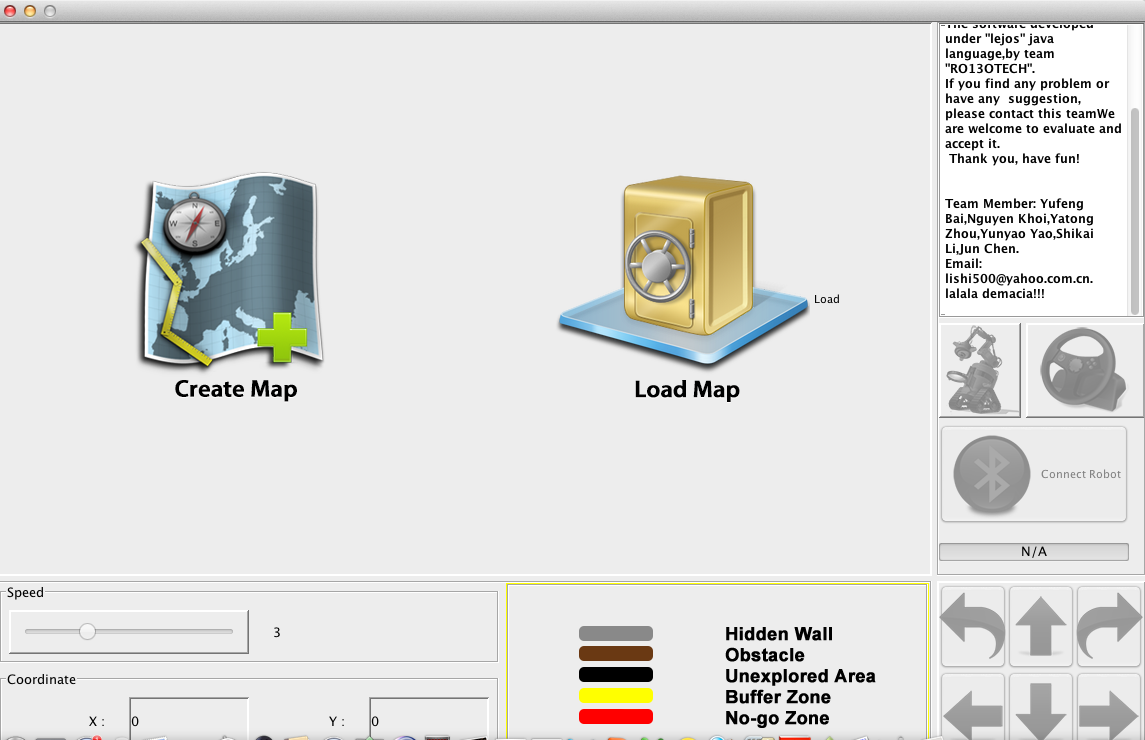
\includegraphics[width=11.20cm]{defaultButton}
\end{center}
\subsection{Pass criteria}
\begin{itemize}
\item The Jbutton.isEnable() methods for addNew, loadMap are true, which means these two buttons are able to be pressed.
\item The Jbutton.isEnable() methods for up, down, left, right, turnLeft, turnRight, auto, manual and bluetoothConnection are false, which means these buttons are not allowed to be pressed.  
\end{itemize}
\subsection{Test Type}
JUnit test
\subsection{Pass or Fail}
Pass

\section{Test2: New map initial button}
\subsection{Description:}
I plan to use Jbutton,doClick() method to implement the operation of creating new map. After confirming the doClick operation, then using Jbutton.isEnabled() method to test the buttons on the GUI screen. The GUI after creating the map shows below:
  \begin{center}
 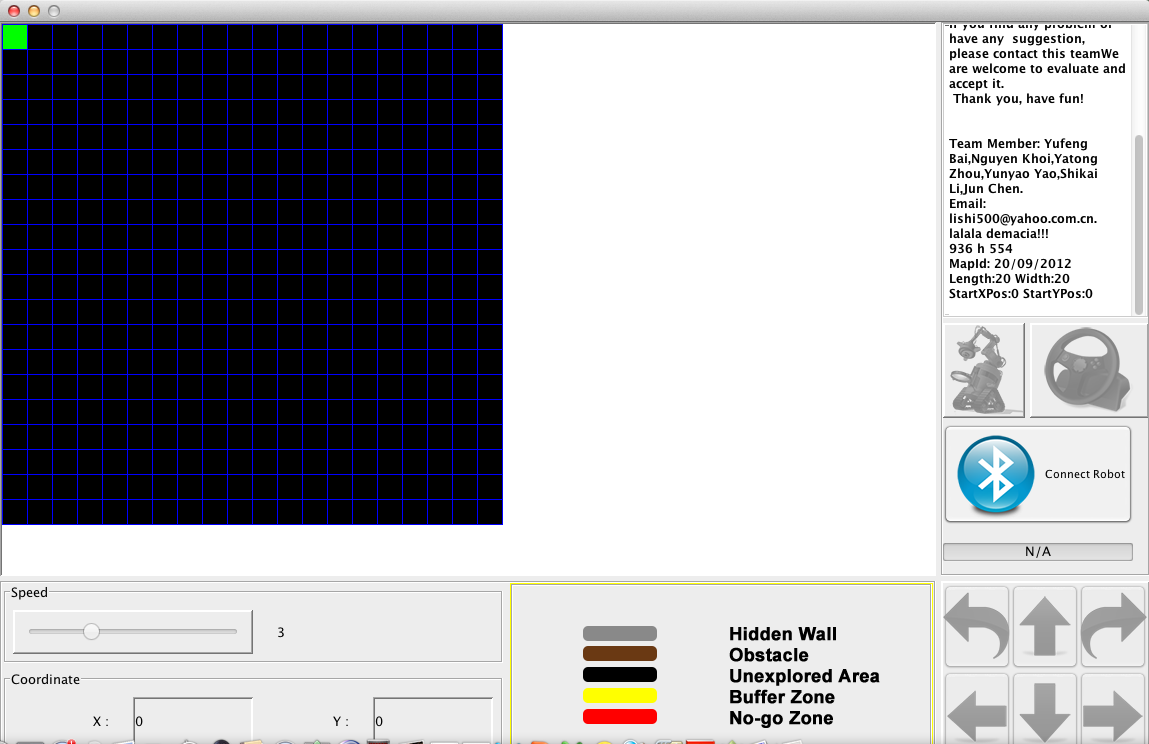
\includegraphics[width=11.20cm]{newmapinitialbutton}
\end{center}
\subsection{Pass criteria}
\begin{itemize}
\item The addNew.doClick() method implements successfully.
\item The Jbutton.isEnable() methods for bluetoothConnection, new map panel are true.
\item The Jbutton.isEnable() methods for loadMap, auto, manual, up, down, left, right, turnLeft, turnRight are not false. 
\end{itemize}
\subsection{Test Type}
JUnit Test
\subsection{Pass or Fail}
Pass
\section{Test3: Bluetooth connection button}
\subsection{Description}
After implementing the addNew.doClick() and bluetoothConnection.doClick() methods, then using Jbutton.isEnabled() method to test the buttons. In addition, if mode change button is pressed, the current mode button is not allowed to be pressed again. The GUI after implementing press the blueConnection button display below:
 \begin{center}
 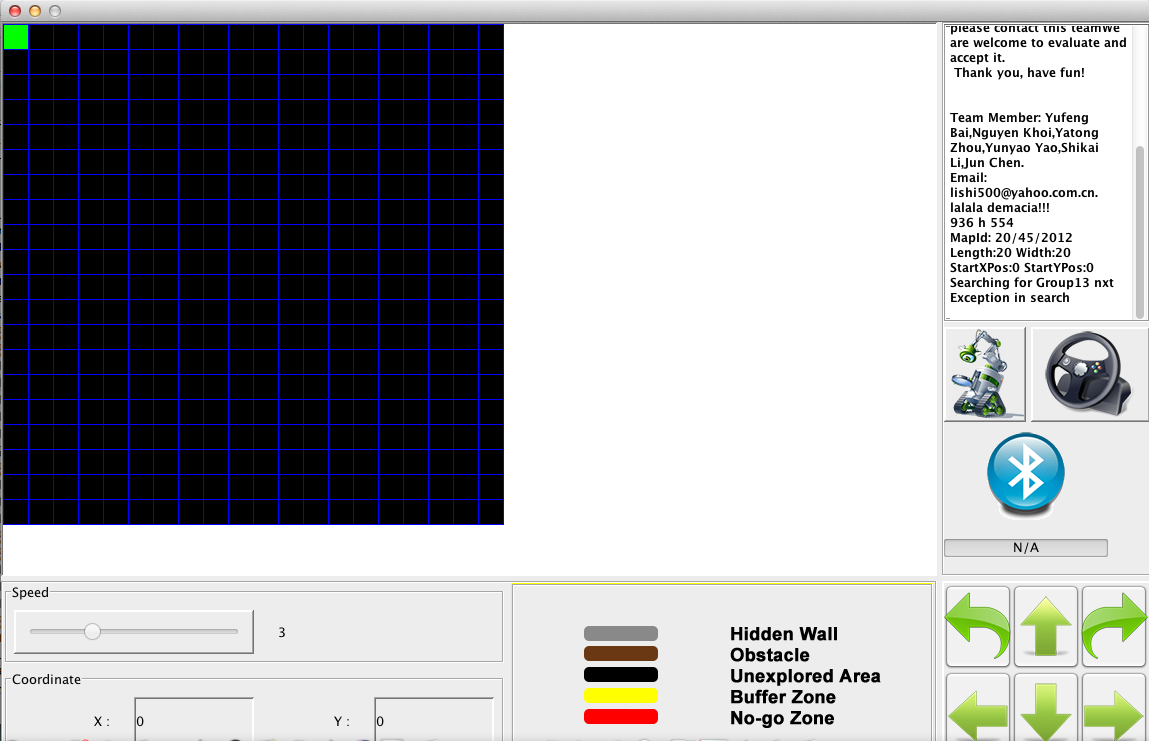
\includegraphics[width=11.20cm]{bluetooth}
\end{center}
\subsection{Pass criteria}
\begin{itemize}
\item The addNew.doClick() and bluetoothConnection.doClick() implements successfully.
\item The Jbutton.isEnabled() methods for auto, manual, up, down, left, right, turnLeft, turnRight are all true
\item After auto.doClick() implements successfully, the Jbutton.isEnabled() method for auto is false
\item After manual.doClick() implements successfully, the Jbutton.isEnabled() method for manual is false
\end{itemize}
\subsection{Test Type}
JUnit Test
\subsection{Pass or Fail}
Pass
\section{Test4: SpeedSlider test}
\subsection{Description}
The initial speed of the robot is 3, when we change the speed of the robot by changing the value on the speed slider, the value beside the speed also will change and this value will display on the robot information board. The speed slider display below:
  \begin{center}
 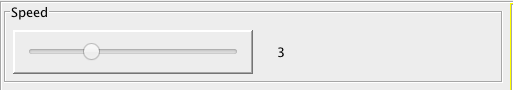
\includegraphics[width=11.20cm]{theinitialspeed}
\end{center}
 \begin{center}
 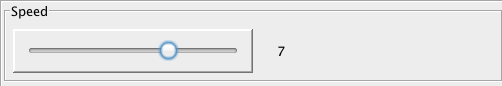
\includegraphics[width=11.20cm]{thechangedspeed}
\end{center}
 \begin{center}
 
\includegraphics[width=11.20cm]{informationboard}
\end{center}
\subsection{Pass criteria}
\begin{enumerate}
\item The initial speed is 3, if user changes the speed, the value beside the speed slider will change immediately.
\item The changed speed will display on the information board. 
\end{enumerate}
\subsection{Test Type}
Junit test
\subsection{Pass or Fail}
Pass
\section{Physical Test1: Forward}
\subsection{Description:}
When the Robot is in manual control mode, when user clicks the arrow which is point to up on GUI one time. The robot is required to move to the north of the map one pixel(the size of pixel is 25mmx25mm).
\subsection{Test Specification}
In my test plan, we decide to paint two pixels(25mmx25mm) on the map by ruler(the sequence of two pixels is up and down). And then place the robot on the paper and make sure the two wheels on the top of line of one pixel. Press the Forward Button one time to make the robot does forward movement. Release the button and record the wheels position on the paper. 
\subsection{Pass Criteria}
\begin{itemize}
\item After the forwarding movement operation, the wheels of the robot is on the top of line of another pixel. 
\end{itemize}
\subsection{Testing Type}
Blackbox
\subsection{Pass or Fail}
Pass
\section{Physical Test2: TurnLeft}
\subsection{Description:}
In manual mode, when user press the turnLeft button, the robot will turn left 90 degrees. This test is to make sure the robot is able to rotate 90 degrees accurately.
\subsection{Test Specification}
In my test plan, I draw a Rectangular Plane Coordinate System on one paper, then place the robot's two wheels on the top of the positive X-coordinate. Pressing the turnLeft button to let the robot implement turn left operation. finally, test whether nor not the robot's wheels on the negative y-coordinate.
\subsection{Pass Criteria}
\begin{itemize}
\item After turning left, the two wheels on the negative y-coordinate of the Rectangular Plane Coordinate System.
\end{itemize}   
\subsection{Testing Type}
Blackbox
\subsection{Pass or Fail}
Pass
\newpage
\appendix
\chapter{the GUI and SpeedSlider test}
The link to the GUI test case is: \\ \\
\url{https://version-control.adelaide.edu.au/svn/sep2012-13/Code/Working%20Copy/Version%200.3/src/Tests/GUITestCase.java}
\begin{lstlisting} 
package Tests;

import static org.junit.Assert.*;

import java.awt.AWTException;
import java.awt.Robot;
import java.awt.event.KeyEvent;

import GUI.*;
import org.junit.Test;

public class GUITestCase {
	LEGOGUI lego;
	@Test
	public void testDefaultButtonEnabled(){
		LEGOGUI lego = new LEGOGUI();
		//test addNew, loadMap initial statues
		assertTrue(lego.addNew.isEnabled());
		assertTrue(lego.loadMap.isEnabled());
		//test auto, manual,bluetoothConnection button initial statues
		assertFalse(lego.auto.isEnabled());
		assertFalse(lego.manual.isEnabled());
		assertFalse(lego.bluetoothConnection.isEnabled());
		
		//test 6 control button initial statues
		assertFalse(lego.up.isEnabled());
		assertFalse(lego.down.isEnabled());
		assertFalse(lego.left.isEnabled());
		assertFalse(lego.right.isEnabled());
		assertFalse(lego.turnLeft.isEnabled());
		assertFalse(lego.turnRight.isEnabled());
		//lego = null;
	}
	
	@Test //(expected = NullPointerException.class)
	public void testNewMapInitialedButtonEnabled(){
		
		// when a new map initialed 
		// test the statues of each button
		 lego = new LEGOGUI();
		
		
		// set addNew map clicked;
		// set new map panel confirm button clicked
		lego.addNew.doClick ();
		lego.nms.mi.Confirm.doClick();
		
		// addNew and loadMap disabled
		assertFalse(lego.loadMap.isEnabled());
		assertTrue(lego.nms.mi.Confirm.isEnabled());
		
		// bluetoothConnection button is enabled
		assertFalse(lego.auto.isEnabled());
		assertFalse(lego.manual.isEnabled());
		assertTrue(lego.bluetoothConnection.isEnabled());
		
		// new map panel is enabled
		assertTrue(lego.nms.mi.isEnabled());	
		lego = null;
		
	}
	@Test //(expected = NullPointerException.class)
	public void testBlueToothConnectedButtonEnabled(){
		lego = new LEGOGUI();
		lego.addNew.doClick ();
		lego.nms.mi.Confirm.doClick();
		//precondition tested through above
		// start connect robot, expected NullPointerException
		lego.bluetoothConnection.doClick();
		// auto and manual Mode enabled
		assertTrue(lego.auto.isEnabled());
		assertTrue(lego.manual.isEnabled());
		// 6 control button enabled
		assertTrue(lego.up.isEnabled());
		assertTrue(lego.down.isEnabled());
		assertTrue(lego.left.isEnabled());
		assertTrue(lego.right.isEnabled());
		assertTrue(lego.turnLeft.isEnabled());
		assertTrue(lego.turnRight.isEnabled());

		//if mode changed 
	lego.auto.requestFocus();
		new Thread(){
        	public void run(){
        		int i = 0;
        		while(i< 10){
        			lego.robot.keyPress(KeyEvent.VK_ENTER);
					try {
						Thread.sleep(100);
					} catch (InterruptedException e) {
						e.printStackTrace();
					}
					i++;
				}
        	}    	
        }.start();

		lego.auto.doClick();
		assertFalse(lego.auto.isEnabled());
		assertTrue(lego.manual.isEnabled());
		lego.manual.doClick();
		assertTrue(lego.auto.isEnabled());
		assertFalse(lego.manual.isEnabled());}

	
	@Test
	public void testSpeedSlider() {
		LEGOGUI lego = new LEGOGUI();
		
		//test speed slider bar reaction and relate label display
		assertEquals(String.valueOf(lego.slider.getValue()), lego.speedLabel.getText().trim());
		
		//test when speed slider is changed
		//if the label is change with it or not
		
		lego.slider.setValue(8);
		assertEquals(String.valueOf(lego.slider.getValue()), lego.speedLabel.getText().trim());
		
		// test when speed is changed, if the textField update the change
		int value = 5;
		String text = lego.text.getText();
		String str = "Speed set to be: " + String.valueOf(value);
		lego.slider.setValue(value);
		assertEquals(String.valueOf(lego.slider.getValue()), lego.speedLabel.getText().trim());
		assertEquals(text+"\n"+str,lego.text.getText());
	}

}
\end{lstlisting}
\chapter{Glossary and Reference}
\section{Glossary}
\begin{itemize}
\item Blackbox: tests the functionality of an application as opposed to its internal structures or workings.
\item GUI: Graphical User Interface.
\item JRE: Java Runtime Environment
\item Junit: is a unit testing framework for the Java programming language.
\end{itemize}
\section{Reference}
\begin{lstlisting} 
http://en.wikipedia.org/wiki/JUnit
http://en.wikipedia.org/wiki/Black-box_testing
http://docs.oracle.com/javase/1.4.2/docs/api/javax/swing/JButton.html
\end{lstlisting} 
\end{document}